\section{Data Acquisition}

%head
The following section will include a description on how the data for the study have been acquired and processed. All data processing, along with GUI design and implementation, will be done in Matlab.

%presentaion of training GUI
To acquire data a training GUI has been designed and implemented in Matlab. The GUI has been designed to fulfil the specific needs for this project. An illustration of the GUI can be seen in \figref{fig:GUI_Training}. 

\begin{figure}[H]
	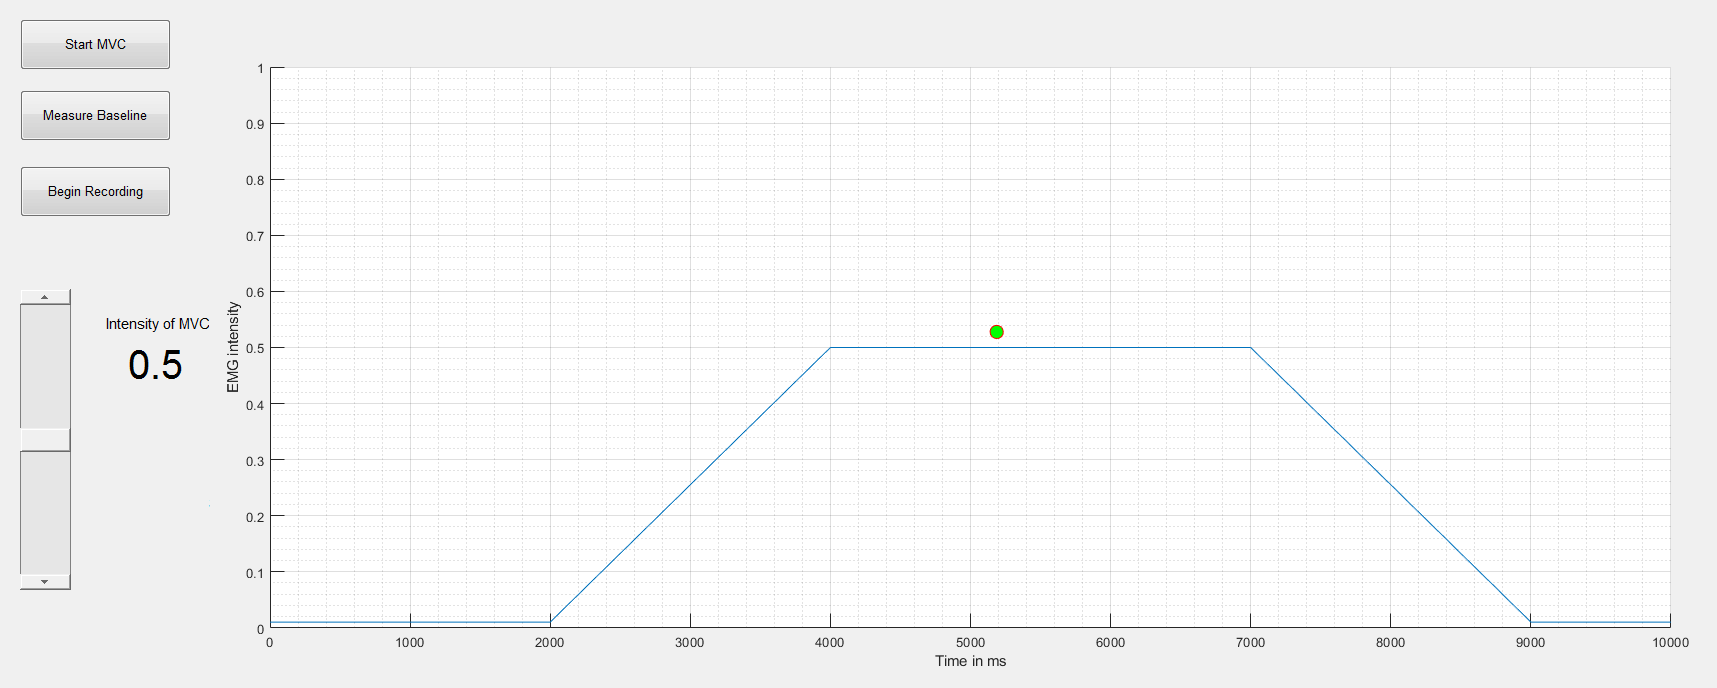
\includegraphics[width=.4\textwidth]{figures/GUI/GUI_Training.png}  %<--but is not needed.
	\caption{\textbf{WE GONNA NEED A NEW PIC OF THE GUI HERE} The training GUI implemented with Matlab GUI development environment. Control buttons to calculate MVC and perform MVC fraction recordings are placed on the left side. The trapezoid plot with the green dot controlled by the input EMG signal from the subject is shown on the right. The fraction of the MVC can be defined by the slider located under the control buttons.}
	\label{fig:GUI_Training}
\end{figure} 

The functions of the GUI consists of a baseline measurement button, a MVC measurement button, a data recording button and a fraction of MVC intensity slider. The baseline measurement is acquired for the purpose of being subtracted from the signal, in order to remove the signal artefacts that are present. At the baseline acquisition the subject is resting the lower arm in the given limb position. The MVC is calculated as a mean of the maximum values in each of the eight channels, and is set as a normalized reference point of 1. The MVC in a contraction at the intensity of which the subject can withhold for 15 seconds. The data recording contains the raw data of a given fraction of the MVC. The fraction is decided by setting a slider to the wanted fraction value, before the recording is started. The slider sets the fraction value so the plateau of the trapeze is at the set value. The trapeze depicts an initial resting phase of two seconds with the intensity of 0, a transition phase of two seconds with an ascending slope until the plateau phase is reached, which has a three second duration, and then a final descending transition phase of two seconds and resting phase of one second. Initialization of the recording will show a green dot, which moves with time on the x-axis and intensity on the y-axis normalized from 0 to 1. The green dot is calculated as the mean of the input EMG signal in a 200 ms window, where each window has an overlap of 100 ms. The signal is afterwards normalized with the MVC measurement as the reference point. From this acquired data features will be extracted and used to train regressors for each of the subjects for each of the hand gestures performed.



%presentation of acquired data

%maybe in the results section(?): differences between the regressors recognizing a movement when they have been trained using log-var and MAV




